% Work of the iterations of a triangular loop (iteration i costs 16 - i units)
% assigned to four threads with three schedules. Generated with a Python script.
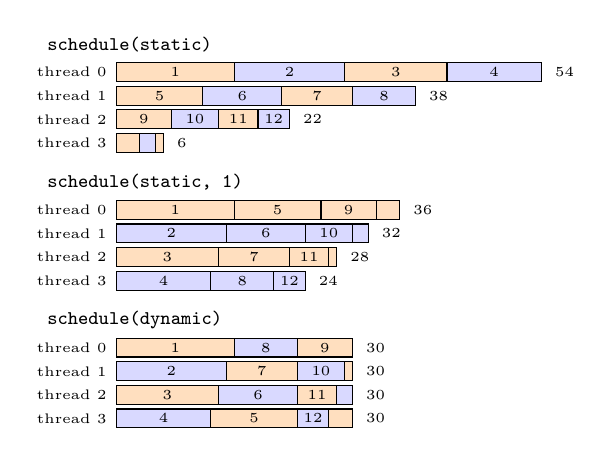
\begin{tikzpicture}[x=1cm, y=1cm]
  \colorlet{c0}{blue!15}
  \colorlet{c1}{orange!25}
  \node[anchor=west, font=\scriptsize] at (-1.0,0.00) {\texttt{schedule(static)}};
  \node[anchor=east, font=\tiny] at (0,-0.35) {thread 0};
  \draw[fill=c1] (0.00,-0.47) rectangle (1.50,-0.23);
  \node[font=\tiny] at (0.75,-0.35) {1};
  \draw[fill=c0] (1.50,-0.47) rectangle (2.90,-0.23);
  \node[font=\tiny] at (2.20,-0.35) {2};
  \draw[fill=c1] (2.90,-0.47) rectangle (4.20,-0.23);
  \node[font=\tiny] at (3.55,-0.35) {3};
  \draw[fill=c0] (4.20,-0.47) rectangle (5.40,-0.23);
  \node[font=\tiny] at (4.80,-0.35) {4};
  \node[anchor=west, font=\tiny] at (5.45,-0.35) {54};
  \node[anchor=east, font=\tiny] at (0,-0.65) {thread 1};
  \draw[fill=c1] (0.00,-0.77) rectangle (1.10,-0.53);
  \node[font=\tiny] at (0.55,-0.65) {5};
  \draw[fill=c0] (1.10,-0.77) rectangle (2.10,-0.53);
  \node[font=\tiny] at (1.60,-0.65) {6};
  \draw[fill=c1] (2.10,-0.77) rectangle (3.00,-0.53);
  \node[font=\tiny] at (2.55,-0.65) {7};
  \draw[fill=c0] (3.00,-0.77) rectangle (3.80,-0.53);
  \node[font=\tiny] at (3.40,-0.65) {8};
  \node[anchor=west, font=\tiny] at (3.85,-0.65) {38};
  \node[anchor=east, font=\tiny] at (0,-0.95) {thread 2};
  \draw[fill=c1] (0.00,-1.07) rectangle (0.70,-0.83);
  \node[font=\tiny] at (0.35,-0.95) {9};
  \draw[fill=c0] (0.70,-1.07) rectangle (1.30,-0.83);
  \node[font=\tiny] at (1.00,-0.95) {10};
  \draw[fill=c1] (1.30,-1.07) rectangle (1.80,-0.83);
  \node[font=\tiny] at (1.55,-0.95) {11};
  \draw[fill=c0] (1.80,-1.07) rectangle (2.20,-0.83);
  \node[font=\tiny] at (2.00,-0.95) {12};
  \node[anchor=west, font=\tiny] at (2.25,-0.95) {22};
  \node[anchor=east, font=\tiny] at (0,-1.25) {thread 3};
  \draw[fill=c1] (0.00,-1.37) rectangle (0.30,-1.13);
  \draw[fill=c0] (0.30,-1.37) rectangle (0.50,-1.13);
  \draw[fill=c1] (0.50,-1.37) rectangle (0.60,-1.13);
  \node[anchor=west, font=\tiny] at (0.65,-1.25) {6};
  \node[anchor=west, font=\scriptsize] at (-1.0,-1.75) {\texttt{schedule(static, 1)}};
  \node[anchor=east, font=\tiny] at (0,-2.10) {thread 0};
  \draw[fill=c1] (0.00,-2.22) rectangle (1.50,-1.98);
  \node[font=\tiny] at (0.75,-2.10) {1};
  \draw[fill=c1] (1.50,-2.22) rectangle (2.60,-1.98);
  \node[font=\tiny] at (2.05,-2.10) {5};
  \draw[fill=c1] (2.60,-2.22) rectangle (3.30,-1.98);
  \node[font=\tiny] at (2.95,-2.10) {9};
  \draw[fill=c1] (3.30,-2.22) rectangle (3.60,-1.98);
  \node[anchor=west, font=\tiny] at (3.65,-2.10) {36};
  \node[anchor=east, font=\tiny] at (0,-2.40) {thread 1};
  \draw[fill=c0] (0.00,-2.52) rectangle (1.40,-2.28);
  \node[font=\tiny] at (0.70,-2.40) {2};
  \draw[fill=c0] (1.40,-2.52) rectangle (2.40,-2.28);
  \node[font=\tiny] at (1.90,-2.40) {6};
  \draw[fill=c0] (2.40,-2.52) rectangle (3.00,-2.28);
  \node[font=\tiny] at (2.70,-2.40) {10};
  \draw[fill=c0] (3.00,-2.52) rectangle (3.20,-2.28);
  \node[anchor=west, font=\tiny] at (3.25,-2.40) {32};
  \node[anchor=east, font=\tiny] at (0,-2.70) {thread 2};
  \draw[fill=c1] (0.00,-2.82) rectangle (1.30,-2.58);
  \node[font=\tiny] at (0.65,-2.70) {3};
  \draw[fill=c1] (1.30,-2.82) rectangle (2.20,-2.58);
  \node[font=\tiny] at (1.75,-2.70) {7};
  \draw[fill=c1] (2.20,-2.82) rectangle (2.70,-2.58);
  \node[font=\tiny] at (2.45,-2.70) {11};
  \draw[fill=c1] (2.70,-2.82) rectangle (2.80,-2.58);
  \node[anchor=west, font=\tiny] at (2.85,-2.70) {28};
  \node[anchor=east, font=\tiny] at (0,-3.00) {thread 3};
  \draw[fill=c0] (0.00,-3.12) rectangle (1.20,-2.88);
  \node[font=\tiny] at (0.60,-3.00) {4};
  \draw[fill=c0] (1.20,-3.12) rectangle (2.00,-2.88);
  \node[font=\tiny] at (1.60,-3.00) {8};
  \draw[fill=c0] (2.00,-3.12) rectangle (2.40,-2.88);
  \node[font=\tiny] at (2.20,-3.00) {12};
  \node[anchor=west, font=\tiny] at (2.45,-3.00) {24};
  \node[anchor=west, font=\scriptsize] at (-1.0,-3.50) {\texttt{schedule(dynamic)}};
  \node[anchor=east, font=\tiny] at (0,-3.85) {thread 0};
  \draw[fill=c1] (0.00,-3.97) rectangle (1.50,-3.73);
  \node[font=\tiny] at (0.75,-3.85) {1};
  \draw[fill=c0] (1.50,-3.97) rectangle (2.30,-3.73);
  \node[font=\tiny] at (1.90,-3.85) {8};
  \draw[fill=c1] (2.30,-3.97) rectangle (3.00,-3.73);
  \node[font=\tiny] at (2.65,-3.85) {9};
  \node[anchor=west, font=\tiny] at (3.05,-3.85) {30};
  \node[anchor=east, font=\tiny] at (0,-4.15) {thread 1};
  \draw[fill=c0] (0.00,-4.27) rectangle (1.40,-4.03);
  \node[font=\tiny] at (0.70,-4.15) {2};
  \draw[fill=c1] (1.40,-4.27) rectangle (2.30,-4.03);
  \node[font=\tiny] at (1.85,-4.15) {7};
  \draw[fill=c0] (2.30,-4.27) rectangle (2.90,-4.03);
  \node[font=\tiny] at (2.60,-4.15) {10};
  \draw[fill=c1] (2.90,-4.27) rectangle (3.00,-4.03);
  \node[anchor=west, font=\tiny] at (3.05,-4.15) {30};
  \node[anchor=east, font=\tiny] at (0,-4.45) {thread 2};
  \draw[fill=c1] (0.00,-4.57) rectangle (1.30,-4.33);
  \node[font=\tiny] at (0.65,-4.45) {3};
  \draw[fill=c0] (1.30,-4.57) rectangle (2.30,-4.33);
  \node[font=\tiny] at (1.80,-4.45) {6};
  \draw[fill=c1] (2.30,-4.57) rectangle (2.80,-4.33);
  \node[font=\tiny] at (2.55,-4.45) {11};
  \draw[fill=c0] (2.80,-4.57) rectangle (3.00,-4.33);
  \node[anchor=west, font=\tiny] at (3.05,-4.45) {30};
  \node[anchor=east, font=\tiny] at (0,-4.75) {thread 3};
  \draw[fill=c0] (0.00,-4.87) rectangle (1.20,-4.63);
  \node[font=\tiny] at (0.60,-4.75) {4};
  \draw[fill=c1] (1.20,-4.87) rectangle (2.30,-4.63);
  \node[font=\tiny] at (1.75,-4.75) {5};
  \draw[fill=c0] (2.30,-4.87) rectangle (2.70,-4.63);
  \node[font=\tiny] at (2.50,-4.75) {12};
  \draw[fill=c1] (2.70,-4.87) rectangle (3.00,-4.63);
  \node[anchor=west, font=\tiny] at (3.05,-4.75) {30};
\end{tikzpicture}
